\section{Introduction}

Hello world! If you are one of those exceptional minds that don't like to use Word, please be welcome and use this \LaTeX template for your project report! A preview of you face in this exact moment is presented in Figure~\ref{fig:example}.

\begin{figure}[h]
    \centering
    
\includegraphics[width=0.25\textwidth]{assets/example.png}
    \caption{Example of a figure from Ref.~\cite{exampleCitation}}
    \label{fig:example}
\end{figure}

\lipsum[1]

\subsection{More}
More information is available for instance at \url{https://www.overleaf.com/learn/latex/Inserting_Images}.

\subsection{Even more}

\lipsum[2]

\subsubsection{More more, maybe?}

\lipsum[3-4]


\subsubsection{This is really the last one}

\lipsum[5]





\section{More but bigger}
Another section.
\ifprintCode
Custom environment \texttt{longlisting} used in Listing~\ref{code:example} enables page breaks within the code snippet.

\subsection{About listings}
More information on code snippets is available for instance at:
\begin{itemize}
    \item \url{https://www.overleaf.com/learn/latex/Code_Highlighting_with_minted},
    \item \href{https://repo.skni.umcs.pl/ctan/macros/latex/contrib/minted/minted.pdf}{minted package documentation.}
\end{itemize}


\begin{longlisting}
\begin{minted}[highlightlines={3}]{python}
import numpy as np
    
def incmatrix(genl1,genl2):
    m = len(genl1)
    n = len(genl2)
    M = None #to become the incidence matrix
    VT = np.zeros((n*m,1), int)  #dummy variable
    
    #compute the bitwise xor matrix
    M1 = bitxormatrix(genl1)
    M2 = np.triu(bitxormatrix(genl2),1) 

    for i in range(m-1):
        for j in range(i+1, m):
            [r,c] = np.where(M2 == M1[i,j])
            for k in range(len(r)):
                VT[(i)*n + r[k]] = 1;
                VT[(i)*n + c[k]] = 1;
                VT[(j)*n + r[k]] = 1;
                VT[(j)*n + c[k]] = 1;
                
                if M is None:
                    M = np.copy(VT)
                else:
                    M = np.concatenate((M, VT), 1)
                
                VT = np.zeros((n*m,1), int)
    
    return M
\end{minted}
\caption{Example code snippet~\cite{code}. \texttt{minted} package is required to compile it.}
\label{code:example}
\end{longlisting}
\fi




\subsection{Use LaTeX beautiful features}


Unlike Word, you can do very fancy stuff with \LaTeX. Please enjoy a vector sketch of a Paul trap...

\begin{center}
\scalebox{1.2}{
    

\tikzset{every picture/.style={line width=0.75pt}} %set default line width to 0.75pt        

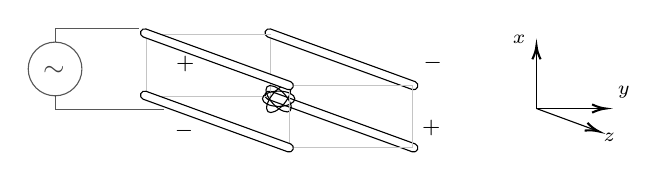
\begin{tikzpicture}[x=0.75pt,y=0.75pt,yscale=-1,xscale=1]
%uncomment if require: \path (0,81); %set diagram left start at 0, and has height of 81

%Rounded Rect [id:dp026469557108133812] 
\draw  [fill={rgb, 255:red, 255; green, 255; blue, 255 }  ,fill opacity=1 ] (125.31,46.91) .. controls (125.69,45.85) and (126.85,45.31) .. (127.91,45.69) -- (197.55,71.04) .. controls (198.6,71.42) and (199.14,72.59) .. (198.76,73.64) -- (198.76,73.64) .. controls (198.38,74.69) and (197.21,75.24) .. (196.16,74.85) -- (126.52,49.51) .. controls (125.47,49.12) and (124.92,47.96) .. (125.31,46.91) -- cycle ;
%Straight Lines [id:da3371385641661644] 
\draw [color={rgb, 255:red, 196; green, 196; blue, 196 }  ,draw opacity=1 ]   (127.91,48.35) -- (127.91,16.69) ;
%Straight Lines [id:da26074727807001774] 
\draw    (256,54) -- (287.37,54) ;
\draw [shift={(289.37,54)}, rotate = 180] [color={rgb, 255:red, 0; green, 0; blue, 0 }  ][line width=0.75]    (6.56,-1.97) .. controls (4.17,-0.84) and (1.99,-0.18) .. (0,0) .. controls (1.99,0.18) and (4.17,0.84) .. (6.56,1.97)   ;
%Straight Lines [id:da32746521719983357] 
\draw    (256,54) -- (256,25.71) ;
\draw [shift={(256,23.71)}, rotate = 90] [color={rgb, 255:red, 0; green, 0; blue, 0 }  ][line width=0.75]    (6.56,-1.97) .. controls (4.17,-0.84) and (1.99,-0.18) .. (0,0) .. controls (1.99,0.18) and (4.17,0.84) .. (6.56,1.97)   ;
%Straight Lines [id:da3165592785302246] 
\draw    (256,54) -- (284.16,64.35) ;
\draw [shift={(286.03,65.04)}, rotate = 200.19] [color={rgb, 255:red, 0; green, 0; blue, 0 }  ][line width=0.75]    (6.56,-1.97) .. controls (4.17,-0.84) and (1.99,-0.18) .. (0,0) .. controls (1.99,0.18) and (4.17,0.84) .. (6.56,1.97)   ;
%Rounded Rect [id:dp23162296971612728] 
\draw  [fill={rgb, 255:red, 255; green, 255; blue, 255 }  ,fill opacity=1 ] (125.31,16.91) .. controls (125.69,15.85) and (126.85,15.31) .. (127.91,15.69) -- (197.55,41.04) .. controls (198.6,41.42) and (199.14,42.59) .. (198.76,43.64) -- (198.76,43.64) .. controls (198.38,44.69) and (197.21,45.24) .. (196.16,44.85) -- (126.52,19.51) .. controls (125.47,19.12) and (124.92,17.96) .. (125.31,16.91) -- cycle ;
%Straight Lines [id:da7801497985171296] 
\draw [color={rgb, 255:red, 196; green, 196; blue, 196 }  ,draw opacity=1 ]   (68.87,18.35) -- (127.91,18.35) ;
%Straight Lines [id:da18932681466243861] 
\draw [color={rgb, 255:red, 196; green, 196; blue, 196 }  ,draw opacity=1 ]   (68.87,48.35) -- (127.91,48.35) ;
%Straight Lines [id:da12487858602452251] 
\draw [color={rgb, 255:red, 196; green, 196; blue, 196 }  ,draw opacity=1 ]   (137.16,72.85) -- (196.2,72.85) ;
%Straight Lines [id:da7561068891818322] 
\draw [color={rgb, 255:red, 196; green, 196; blue, 196 }  ,draw opacity=1 ]   (137.12,42.85) -- (196.16,42.85) ;
%Straight Lines [id:da36016830120348087] 
\draw [color={rgb, 255:red, 196; green, 196; blue, 196 }  ,draw opacity=1 ]   (67.91,48.35) -- (67.91,16.69) ;
%Straight Lines [id:da6626175855941887] 
\draw [color={rgb, 255:red, 196; green, 196; blue, 196 }  ,draw opacity=1 ]   (196.16,72.85) -- (196.16,42.85) ;
%Shape: Ellipse [id:dp4879513077667338] 
\draw   (123.97,49.28) .. controls (123.97,47.25) and (127.46,45.6) .. (131.77,45.6) .. controls (136.08,45.6) and (139.58,47.25) .. (139.58,49.28) .. controls (139.58,51.32) and (136.08,52.97) .. (131.77,52.97) .. controls (127.46,52.97) and (123.97,51.32) .. (123.97,49.28) -- cycle ;
%Shape: Ellipse [id:dp6977784877320135] 
\draw   (126.61,55.48) .. controls (125.17,54.14) and (126.31,50.27) .. (129.16,46.85) .. controls (132.02,43.42) and (135.5,41.74) .. (136.94,43.09) .. controls (138.38,44.43) and (137.24,48.3) .. (134.38,51.72) .. controls (131.53,55.15) and (128.05,56.83) .. (126.61,55.48) -- cycle ;
%Shape: Ellipse [id:dp4347278984290077] 
\draw   (126.2,43.5) .. controls (127.54,42.05) and (131.13,43.46) .. (134.21,46.65) .. controls (137.29,49.85) and (138.7,53.62) .. (137.35,55.07) .. controls (136,56.52) and (132.42,55.11) .. (129.34,51.92) .. controls (126.26,48.72) and (124.85,44.95) .. (126.2,43.5) -- cycle ;

%Straight Lines [id:da9283418522076294] 
\draw [color={rgb, 255:red, 196; green, 196; blue, 196 }  ,draw opacity=1 ]   (137.16,73.85) -- (137.16,42.2) ;
%Rounded Rect [id:dp4934943713792619] 
\draw  [fill={rgb, 255:red, 255; green, 255; blue, 255 }  ,fill opacity=1 ] (65.31,16.91) .. controls (65.69,15.85) and (66.85,15.31) .. (67.91,15.69) -- (137.55,41.04) .. controls (138.6,41.42) and (139.14,42.59) .. (138.76,43.64) -- (138.76,43.64) .. controls (138.38,44.69) and (137.21,45.24) .. (136.16,44.85) -- (66.52,19.51) .. controls (65.47,19.12) and (64.92,17.96) .. (65.31,16.91) -- cycle ;
%Rounded Rect [id:dp8209197314293472] 
\draw  [fill={rgb, 255:red, 255; green, 255; blue, 255 }  ,fill opacity=1 ] (65.31,46.91) .. controls (65.69,45.85) and (66.85,45.31) .. (67.91,45.69) -- (137.55,71.04) .. controls (138.6,71.42) and (139.14,72.59) .. (138.76,73.64) -- (138.76,73.64) .. controls (138.38,74.69) and (137.21,75.24) .. (136.16,74.85) -- (66.52,49.51) .. controls (65.47,49.12) and (64.92,47.96) .. (65.31,46.91) -- cycle ;
%Shape: Circle [id:dp9266584324169199] 
\draw  [color={rgb, 255:red, 0; green, 0; blue, 0 }  ,draw opacity=0.66 ] (11.13,34.93) .. controls (11.13,27.79) and (16.92,22) .. (24.07,22) .. controls (31.21,22) and (37,27.79) .. (37,34.93) .. controls (37,42.08) and (31.21,47.87) .. (24.07,47.87) .. controls (16.92,47.87) and (11.13,42.08) .. (11.13,34.93) -- cycle ;
%Straight Lines [id:da6054328790639063] 
\draw [color={rgb, 255:red, 0; green, 0; blue, 0 }  ,draw opacity=0.66 ]   (24.07,22) -- (24.07,15.53) ;
%Straight Lines [id:da8018312921143852] 
\draw [color={rgb, 255:red, 0; green, 0; blue, 0 }  ,draw opacity=0.66 ]   (24.07,15.53) -- (64.67,15.53) ;
%Straight Lines [id:da3703100332961291] 
\draw [color={rgb, 255:red, 0; green, 0; blue, 0 }  ,draw opacity=0.66 ]   (24.07,54.33) -- (24.07,47.87) ;
%Straight Lines [id:da6734660603789357] 
\draw [color={rgb, 255:red, 0; green, 0; blue, 0 }  ,draw opacity=0.66 ]   (24.07,54.33) -- (76.67,54.33) ;

% Text Node
\draw (243.33,17.6) node [anchor=north west][inner sep=0.75pt]  [font=\scriptsize]  {$x$};
% Text Node
\draw (294,42.07) node [anchor=north west][inner sep=0.75pt]  [font=\scriptsize]  {$y$};
% Text Node
\draw (287.13,64.73) node [anchor=north west][inner sep=0.75pt]  [font=\scriptsize]  {$z$};
% Text Node
\draw (81.13,27.53) node [anchor=north west][inner sep=0.75pt]  [font=\footnotesize]  {$+$};
% Text Node
\draw (199.6,58.2) node [anchor=north west][inner sep=0.75pt]  [font=\footnotesize]  {$+$};
% Text Node
\draw (80.53,59.93) node [anchor=north west][inner sep=0.75pt]  [font=\footnotesize]  {$-$};
% Text Node
\draw (200.4,26.8) node [anchor=north west][inner sep=0.75pt]  [font=\footnotesize]  {$-$};
% Text Node
\draw (17.0,32.53) node [anchor=north west][inner sep=0.75pt]  [color={rgb, 255:red, 0; green, 0; blue, 0 }  ,opacity=0.75 ]  {$\sim$};


\end{tikzpicture}


}
\end{center}
... or this stunning Lindblad equation
\begin{equation}
    \dot{\rho} = \frac{i}{\hbar} [\rho,H] + \sum_j \gamma_j \left( L_j \, \rho \,  L_j^\dagger - \frac{1}{2} \Bigl\{ L_j^\dagger L_j, \, \rho \Bigr\} \right)
    \label{eq:Lindblad}
\end{equation}





% Use \section*{REFERENCES} to avoid REFERENCES being shown in the table of contents
\section*{REFERENCES}
\printbibliography[heading=none]

\noindent More information on bibliography is available for instance at \url{https://www.overleaf.com/learn/latex/Bibliography_management_with_biblatex}.

